% ===================================================================================== %
%                                        Header                                         %
% ===================================================================================== %
\documentclass[10pt,t,xcolor=table]{UWMadBeamer}

\usepackage{textcomp}
\usepackage{setspace}
\usepackage{booktabs}
\usepackage{multirow}


\newenvironment{Itemize}
    {\begin{itemize}\setlength{\itemsep}{0.50em}\setlength{\leftmargin}{0.0em}\setlength{\labelwidth}{0em}}
    {\end{itemize}}



%\title{On the Stability of Natural Circulation Loops with Phase Change}
\Title{Version Control Introduction}
\Institute{University of Wisconsin--Madison}
\Department{Engineering Physics Department}
\Author{Troy C. Haskin}
\date{5/12/2014}

\AtBeginSection[]{
    \begin{frame}<beamer>
        \tableofcontents[currentsection]
    \end{frame}
}
\AtBeginSubsection[]{
    \ifnum\value{subsection} > 1
        \begin{frame}<beamer>
            \tableofcontents[currentsection,currentsubsection]
        \end{frame}
    \fi
}


\graphicspath{{./Graphics/}}


% =========================================================================== %
%                              Document                                       %
% =========================================================================== %
\begin{document}


% ======================================================= %
%                         Titlepage                       %
% ======================================================= %
\section{Start}
\begin{frame}
    \titlepage
\end{frame}


% ======================================================= %
%                         Outline                         %
% ======================================================= %
\begin{frame}
    \tableofcontents
\end{frame}



% ======================================================= %
%                         Motivation                      %
% ======================================================= %
\section{Motivation}

    \subsection{Paper Example}

    \begin{frame}{Paper Workflow}
        A typical workflow of writing a paper:
        \begin{Itemize}
            \item{Start with an idea/outline}
            \item{Make a draft}
            \item{Proof}
            \item{Edit}
            \item{Repeat until done}
        \end{Itemize}
    \end{frame}

    \begin{frame}{Workflow Shortcomings}
        Individual paper:
        \begin{Itemize}
            \item{Forget what changes were and were not made}
            \item{Make big changes but like the way it was}
            \item{Want to use the material again but alter for a different audience, journal, etc.}
        \end{Itemize}
        
        Group paper:
        \begin{Itemize}
            \item{Don't know what changes were and were not made}
            \item{Not sure what version of the paper you or others have}
            \item{Not sure who or what was added to the version in-use}
        \end{Itemize}
    \end{frame}

    \begin{frame}{Solution}
        A common solution not using a version control system (VCS):

        \begin{Itemize}
            \item{Make a new directory and name appropriately}
            \begin{Itemize}
                \item{\texttt{NuclearEngineeringAndDesign}}
                \item{\texttt{AnnalsOfNuclearEnergy}}
            \end{Itemize}
            \item{Make a new copy of the file and name it something different}
            \begin{Itemize}
                \item{\texttt{AwesomePaper-Draft1.docx}}
                \item{\texttt{AwesomePaper-AdvisorsNotes.docx}}
                \item{\texttt{AwesomePaper-Draft2NeedCitations.docx}}
                \item{\texttt{AwesomePaper-Final.docx}}
                \item{\texttt{AwesomePaper-FinalAdvisorNotes.docx}}
                \item{\texttt{AwesomePaper-FinalFinal.docx}}
            \end{Itemize}
        \end{Itemize}
    \end{frame}

    \begin{frame}{Solution Shortcomings}
        \begin{Itemize}
            \item{Proliferation of files and directories}
            \item{No automatic list of changes; ``proper'' naming attempts to correct this (\eg{}, \texttt{Draft2NeedCitations})}
            \item{Ability to go back to an earlier version would complicate naming}
            \item{Collaboration issues still not addressed}
        \end{Itemize}
    \end{frame}

    \subsection{Other Examples}

    \begin{frame}{RELAP/MELCOR Inputs:}
        \begin{Itemize}
            \item{Build the model by slowly adding control volumes and heat structures}
            \item{Adjust geometry input as more information becomes available}
            \item{Correct issues as they're discovered}
            \item{Might break things and need to find a older, working version}
            \item{\textbf{Re-use the input for multiple different simulations or numerical experiments}}
        \end{Itemize}
    \end{frame}


    \begin{frame}{Writing Programs}
        \begin{Itemize}
            \item{Start simple and add more functionality}
            \item{Fix bugs as they're discovered}
            \item{Might break things and need to find a older, working version}
            \item{Someone else might want to leap off of the work already done but apply it differently}
        \end{Itemize}
    \end{frame}

    \begin{frame}{Same Problems}
        \begin{Itemize}
            \item{These examples, and many more, all have the problems presented by the paper example.}
            \item{The problems only become worse as the work becomes larger or more people become involved.}
        \end{Itemize}
        
        What's the solution?
    \end{frame}



% ======================================================= %
%                   Version Control System                %
% ======================================================= %
\section{Version Control System}

    \subsection{Introduction}
    \begin{frame}{What is it?}
        \begin{description}
            \item
                [{\usebeamercolor[fg]{frametitle} Definition}]
                {A system that records changes to a file or set of files over time so that you can recall specific versions later.}
                \textsuperscript
                    {{\usebeamercolor
                        [fg]{frametitle}
                        \href
                            {http://git-scm.com/book/en/Getting-Started-About-Version-Control}
                            {src}}}
        \end{description}
        
        Features:
        \begin{Itemize}
            \item{Revert a file or an entire project back to a previous state}
            \item{Review changes made over time}
            \item{See who last modified something}
            \item{Create an off-shoot from a current project state (branching)}
            \item{Create a brand new project from a current project (forking)}
            \item{Work locally and save to an online system (distributed systems)}
        \end{Itemize}
    \end{frame}

    \begin{frame}{Advantages / Disadvantages}
        Advantages
        \begin{Itemize}
            \item{History of the project is automatically cataloged}
            \item{All versions of the project are saved and ID-ed automatically}
            \item{Line-by-line and person-by-person reviewable history.}
        \end{Itemize}
        
        Disadvantages:
        \begin{Itemize}
            \item{Can't see line-by-line changes for binary files (\eg{}, \texttt{docx} or image files)}
            \item{Not good for saving humongous files (large binary data files shouldn't be versioned)}
            \item{Requires discipline and effort to log and sync changes}
            \item{Becomes much, much more complicated for larger projects (not a worry for us)}
        \end{Itemize}
    \end{frame}


    \subsection{How it Works}
    \begin{frame}{Definitions {\small (Examples to follow)}}
        \begin{description}
            \setlength{\itemsep}{0.65em}
            \item[{\usebeamercolor[fg]{frametitle} Repository}]
                {A directory that holds all project files and VCS information.}
            \item[{\usebeamercolor[fg]{frametitle} Commit}]
                {A submission of changes from the user to the VCS; this creates a new version and saves the previous state in the history}
            \item[{\usebeamercolor[fg]{frametitle} Commit Message}]
                {A short/long description of the changes present in the commit.}
            \item[{\usebeamercolor[fg]{frametitle} Branch}]
                {A new, separate line of history starting from a certain version; changes can be made to a branch without affecting what it was branched from}
            \item[{\usebeamercolor[fg]{frametitle} Diff}]
                {A comparison of two files with line-by-line differences highlighted}
            \item[{\usebeamercolor[fg]{frametitle} Sync/Push}]
                {A synchronization of a local repository with a non-local one}
        \end{description}
    \end{frame}

    \begin{frame}{History/Commit Example}
        \begin{columns}[T]
            \begin{column}[T]{0.48\textwidth}
                \centering
                    \includegraphics<1>[scale=0.43]{Workflow1}
                    \includegraphics<2>[scale=0.43]{Workflow2}
                    \includegraphics<3>[scale=0.43]{Workflow3}
                    \includegraphics<4>[scale=0.43]{Workflow4}
            \end{column}
            \begin{column}[T]{0.48\textwidth}
                History:
                \begin{enumerate}
                    \item<2->{'Notes.txt' created.}
                    \item<3->{Added new note to 'Notes.txt'.}
                    \item<4->{Added new file 'Classes.txt'. }
                \end{enumerate}

                \only<1>{\hfill\textit{REPO Info. initially empty}}
            \end{column}
        \end{columns}
    \end{frame}

    \begin{frame}{History of This Presentation}
        \centering
        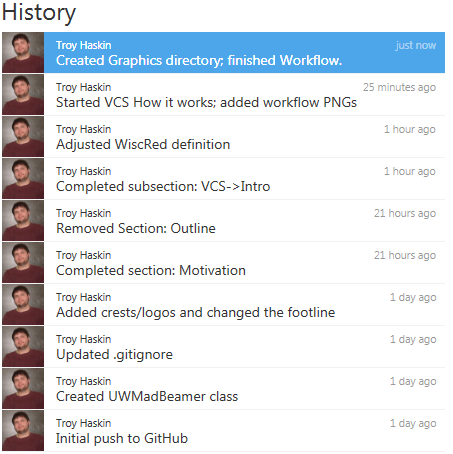
\includegraphics[scale=0.40]{VCSHistoryExample}
    \end{frame}

    \begin{frame}[c]{Branching Example}
        Branches share a common ancestor but can have different histories after the branch commit.

        {
            \centering
            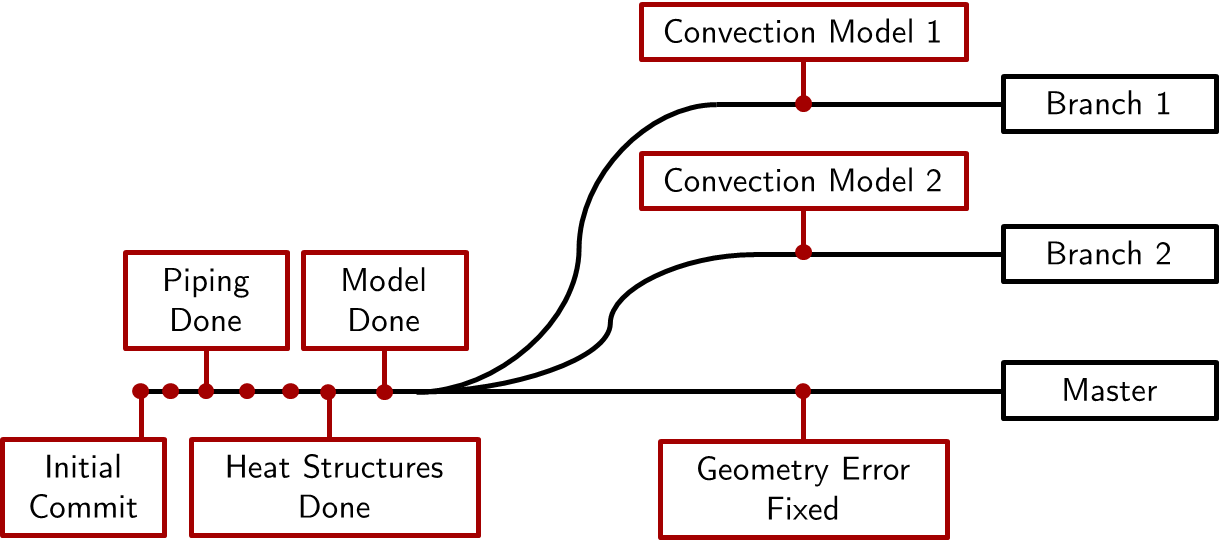
\includegraphics[scale=0.52]{BranchExample}
        }
    \end{frame}

    \begin{frame}[c]{Merge Example}
        It is possible to {\usebeamercolor[fg]{frametitle}merge} histories in branches but can lead to {\usebeamercolor[fg]{frametitle} conflicts} (mismatched or ambiguous histories that require resolution).
        
        {
            \centering
            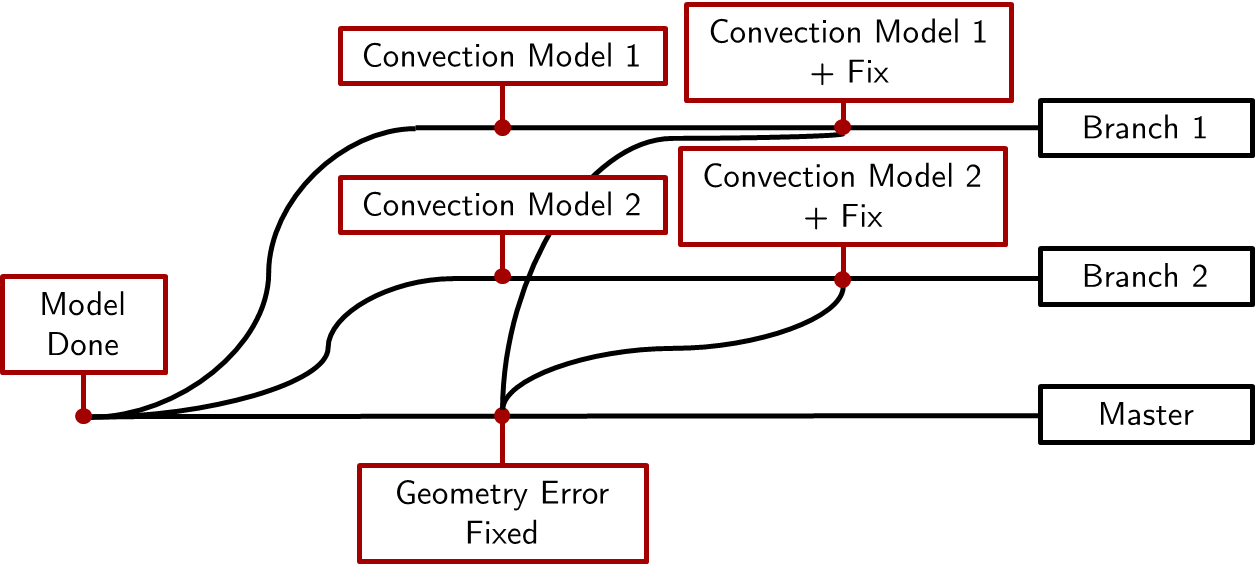
\includegraphics[scale=0.50]{MergeExample}
        }
    \end{frame}

    \begin{frame}{Ignoring Files}
        As was stated before, versioning large binary files is not good practice.
        Large restart or plot files should be stored elsewhere.
        \vfill
        In order to accomplish this, all VCSs have a manner of ignoring files.
        \vfill
        For Git, what we will cover next, it involves editing the \texttt{.gitignore} file.
    \end{frame}

    \begin{frame}{That's it}
        And that covers the broad introduction.
        
        There is more, of course, but that will wait for later.
    \end{frame}



% ======================================================= %
%                     Git and GitHub                      %
% ======================================================= %
\section{Git and GitHub}

    \subsection{}
    \begin{frame}{The Program and the Website}
        \begin{description}
            \setlength{\itemsep}{0.65em}
            \item[{\usebeamercolor[fg]{frametitle} Git}]
                {My VCS program of choice; created to manage one of the largest collaborative projects in history --- the Linux Kernel.}
            \item[{\usebeamercolor[fg]{frametitle} GitHub}]
                {A website the allows online hosting of repositories and uses Git as its VCS.  Public repositories are completely free; private repositories cost money.}
        \end{description}
    \end{frame}


    \subsection{}
    \begin{frame}{GitHub Applications}
        \begin{description}
            \setlength{\itemsep}{0.65em}
            \item[{\usebeamercolor[fg]{frametitle} GitHubWindows}]
                {An application for Windows 7/8 that syncs repositories between a computer and GitHub}
            \item[{\usebeamercolor[fg]{frametitle} GitHubMac}]
                {An application for OSX 10.7+ that syncs repositories between a computer and GitHub}
        \end{description}
        Both programs allow for creation, commits, branching, merging, and more.
    \end{frame}

    \subsection{}
    \begin{frame}[c]{My GitHub For Windows}
        \includegraphics<1>[scale=0.2125]{GitHubForWindowsMain}
        \includegraphics<2>[scale=0.2125]{GitHubForWindowsVCS}
    \end{frame}


\section{End}
    \begin{frame}{Thank You!}

        Links:
        \begin{Itemize}
            \setlength{\itemsep}{2em}
            \item   {
                \usebeamercolor[fg]{frametitle}
                \href{https://github.com/troyhaskin} {Troy's GitHub Page}
            }
            \item   {
                \usebeamercolor[fg]{frametitle}
                \href{https://github.com/ThermalHydraulicsLab} {THL's GitHub Page}
            }
            \item   {
                \usebeamercolor[fg]{frametitle}
                \href{https://windows.github.com/} {GitHubWindows}
            }
            \item   {
                \usebeamercolor[fg]{frametitle}
                \href{https://mac.github.com/} {GitHubMac}
            }
            \item   {
                \usebeamercolor[fg]{frametitle}
                \href{https://raw.githubusercontent.com/ThermalHydraulicsLab/UWMadisonExperiment-RELAP5/master/.gitignore} {RELAP/MELCOR \texttt{.gitignore} file}
            }
        \end{Itemize}

    \end{frame}

\end{document}

